\section{Convergence Analysis}

Now down to the main point, we would like to analyze and confirm the convergence
of the Parareal method. First we derive a theoretical result, and then confirm
it through numerical expirements.

\subsection{Theoretical Convergence}

Suppose we have the following ordinary differential equation:

\begin{equation}
  \begin{cases}
    u' = f(t,u), \quad t > 0 \\
    u(0) = u_0
  \end{cases}
\end{equation}

In addition suppose we have the course operator $\course(t^{n+1},t^n,u^n)$ and
the fine operator $\fine(t^{n+1}, t^n, u^n)$ with the following properties:

\begin{enumerate}
  \item On $\course(t^{n+1},t^n,u^n)$:
    \begin{itemize}
      \item Suppose this operator has order $m$.
      \item Suppose it's Lipschitz in the initial condition:
        \[
          \norm{\course(t^{n+1},t^n,u)-\course(t^{n+1},t^n,v)} \leq 
          C\norm{u - v} 
        \]
        In particular we write $C = (1 + L \Delta t)$.
    \end{itemize}
  \item With respect to $\fine(t^{n+1}, t^n, u^n)$, we suppose it's accurate
    enough to be assumed to be the true solution $u^*$. This means that if
    $\course$ is accurate with order $m$ to the true solution, then it too will
    be so to $\fine$.
\end{enumerate}

Then we can prove the following theorem:

\begin{theorem*}
  The parareal method with course operator $\course$ and fine operator $\fine$
  has order of accuracy $mk$, where $k-1$ is the number of parareal iterations
  made. \cite{balarticle} \cite{fieldstalk}
\end{theorem*}
\begin{proof}
  We proceed via induction on $k$ and $n$. Suppose $k = 1$, then it is trivial,
  this is the course operator, and for $n = 0$, this is the initial condition
  which we know to any accuracy.

  Now suppose for $k,n > 1$, that we know:
  \[
    \norm{u(t^n) - u_k^n} \leq \norm{u_0}C(\Delta t)^{mk}, 
  \]
  We want to show that:
  \[
    \norm{u(t^n) - u_{k+1}^n} \leq \norm{u_0}C(\Delta t)^{m(k+1)}
  \]
  To proceed, recall that $\fine$ is assumed to be a good approximation for
  $u(t^n)$, so we may write:
  \begin{align*}
    \norm{u(t^n) - u_{k+1}^n} & = \norm{\fine(u(t^{n-1})) -
    \course(u^{n-1}_{k+1}) - \fine(u^{n-1}_k) + \course(u^{n-1}_k)} \\
    & = \norm{\course(u(t^{n-1})) + \delta \course (u(t^{n-1}))  -
    \course(u^{n-1}_{k+1}) - \delta \course(u^{n-1}_k)} \\
    & \leq \norm{\course(u(t^{n-1})) - \course(u^{n-1}_{k+1})} + 
    \norm{ \delta \course (u(t^{n-1})) - \delta \course(u^{n-1}_k)} \\
    & \leq (1+L\Delta t)\norm{u(t^{n-1}) - u^{n-1}_{k+1}} + 
    C(\Delta t)^{m+1}\norm{ u(t^{n-1}) - u^{n-1}_k} \\
    & \leq (1+L\Delta t)\norm{u(t^{n-1}) - u^{n-1}_{k+1}} + 
    C(\Delta t)^{m+1}(\Delta t)^{mk}\norm{ u_0 } \\
    & \leq (1+L\Delta t)\norm{u(t^{n-1}) - u^{n-1}_{k+1}} + 
    C(\Delta t)^{m(k+1)+1}\norm{ u_0 } \\
  \end{align*}
  At this point, note that the left hand term is the approximation of $u$ at the
  previous time step, which we can assume to also be of the order $m(k+1)$.
  Therefore, we can say that $\norm{u(t^n) - u_{k+1}^n} = \mathcal{O}(\Delta
  t^{m(k+1)})$, completing our inductive step.
\end{proof}

\subsection{Numerical Results and Validation}

Here we seek to confirm the theoretical order derived in the last section (from
\cite{balarticle} \cite{fieldstalk}). To see a clear example, consier the Euler
methods introduced back in section \ref{sec:euler}. Recall that the explicit
Euler method is of order $1$, so theoretically if we have a fine method of high
enough order, we should see a method whose order is $k$, for an order $k$
Parareal. And indeed, as we expect, we do indeed see such such results, see
figure \ref{fig:conv_fw} for the numerical plots.

\begin{figure}[!htb]
  \centering
  \begin{subfigure}{\textwidth}
    \centering
    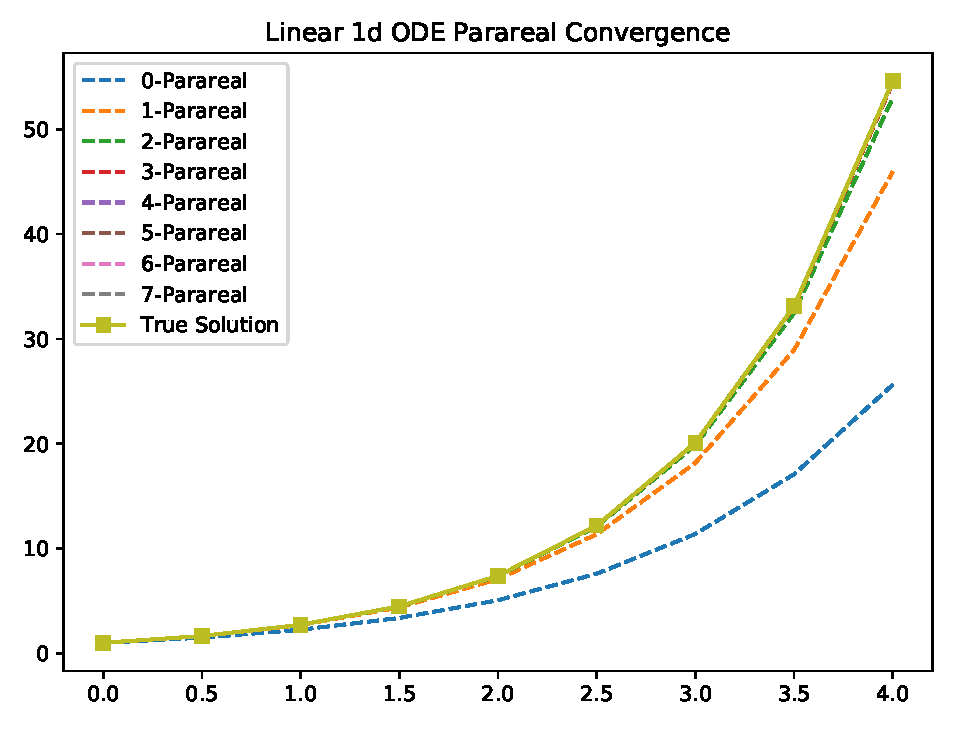
\includegraphics[width=.515\textwidth]
      {./resources/converge_fwsols}
    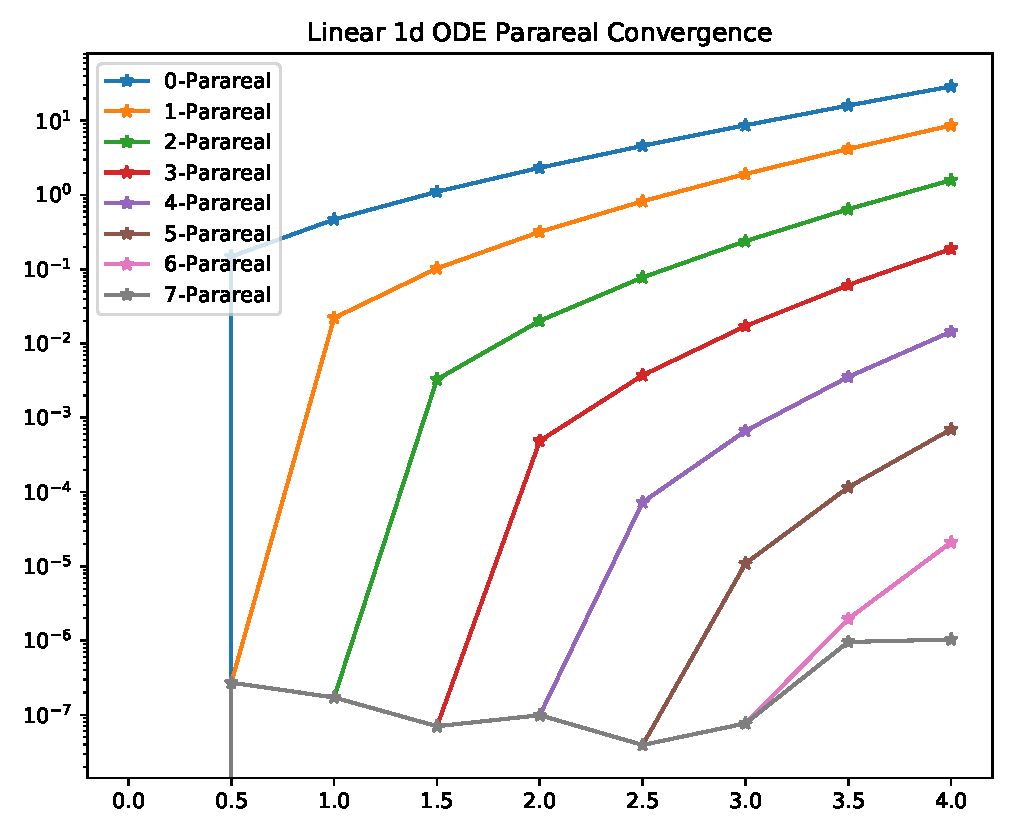
\includegraphics[width=.475\textwidth]
      {./resources/converge_fwerrs}
  \end{subfigure}%
  \caption{The figure on the left is showing the resulting solutions to the ODE
    $u' = u, u(0) = 1$ for $t \in [0, 4]$, and the right is showing the errors
    under the $1$ norm. Critically, this plot reveals that our implementation of
    Parareal conforms to the theoreical convergence rate, which validates our
    method. The last iterate has strange behavior, but this is because I could
    not decrease the accuracy of the fine integrator (forward Euler) anymore
    without running out of memory.}\label{fig:conv_fw}
\end{figure}

Using this information, we might begin to consider how can we leverage this $mk$
convergence rate. It's immediately clear, that if we want $k$ to be as small as
possible (as noted in the efficiency section), that we want $m$ to be as large
as possible. However, $m$ corresponds to the order of the course integrator, and
typically we want this integrator to be as cheap and inexpensive as possible.
Therefore, we have an optimization problem here between the course integrator
and number of parareal iterations. Of course, all of this is assuming that the
fine integrator performs to the desired accuracy, otherwise the former is
useless. 

For example, see figure \ref{fig:conv_rk} for a examination of the errors of
parareal underneath the Runge-Kutta methods. In addition, see figure
\ref{fig:order_conf} for a more confirmation of the $mk$ order, for the
Runge-Kutta methods.

\begin{figure}[!htb]
  \centering
  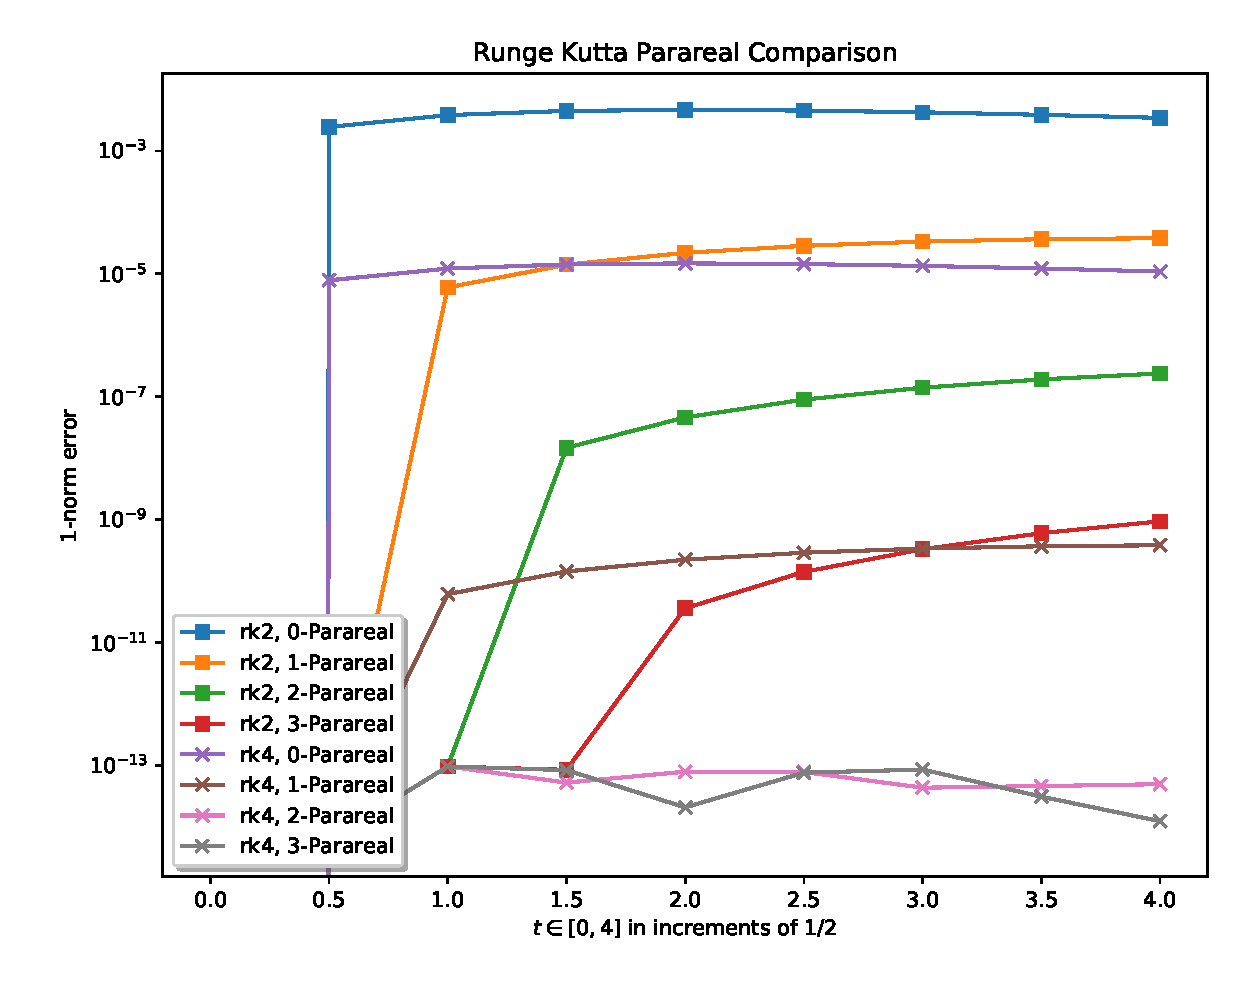
\includegraphics[width=.85\textwidth]{./resources/runge_kutta_parareal}
  \caption{This figure is showing the resulting errors in the parareal
    approximation to to the ODE $u' = -\frac{1}{2}u, u(0) = 1$ for $t \in [0,
    4]$ under the $1$ norm. This plot reveals how, given a higher order course
    method, the parareal is able to make larger jumps of accuracy as the number
    of parareal iterations increases.}\label{fig:conv_rk}
\end{figure}

\begin{figure}[!htb]
  \centering
  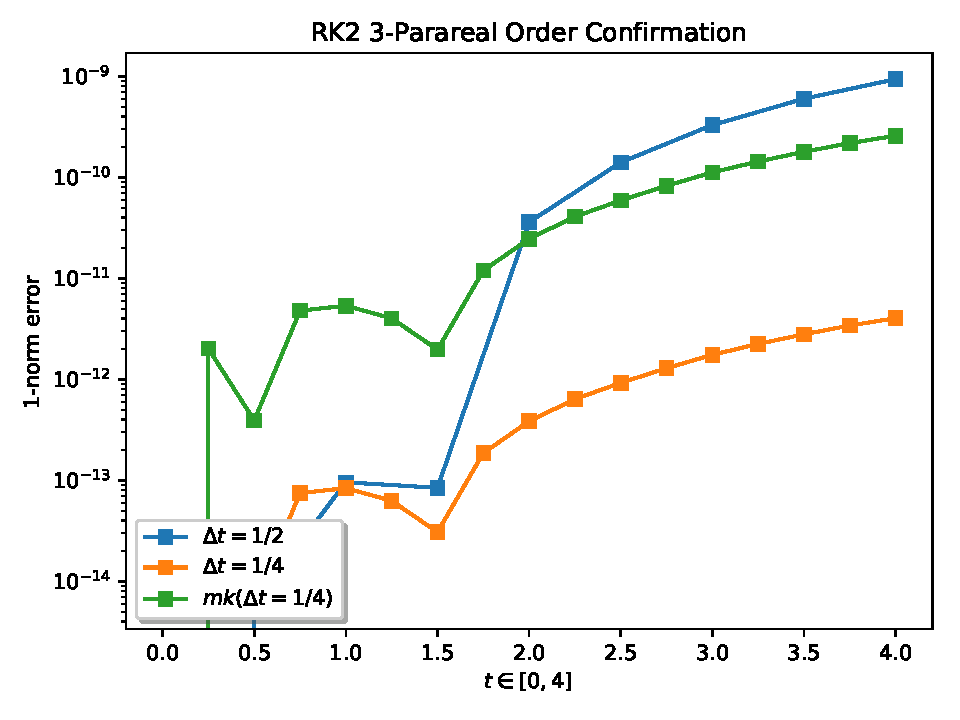
\includegraphics[width=.75\textwidth]{./resources/rk2_order_conf}
  \caption{This figure shows that how, under refinement of $\Delta t$, the third
    parareal iteration of the Runge Kutta $2$ method has order roughly
    $5$. This is confirmed by taking the error of $\Delta t/2$ and shifting it
    by the order. They don't exactly land on top of each other, but I believe
    that to be an artifact of the approximation not being exact.}\label{fig:order_conf}
\end{figure}
